% Harmadik előadás

\chapter{Disszipációkezelés}

\section{A disszipációkezelés fontossága}
A processzorok fejlesztésének két iránya van: teljesítmény növelése és a fogyasztás csökkentése.
A fejlesztés fókusza folyamatosan a disszipáció csökkentése felé tolódott, mivel rájöttek, hogy a teljesítmény fő korlátja a disszipáció.

\section{A disszipáció}
A disszipáció két komponensből áll: dinamikus (működés közbeni) és statikus.
A tápegység szempontjából a processzor egy szórt kapacitás, amit a felfutó órajelen fel kell tölteni, a lefutón pedig egy ellenálláson keresztül le kell vezetni.
A töltés-kisülés fogyasztása a dinamikus disszipáció.
A statikus disszipáció a lezárt tranzisztorok szivárgási áramából adódik.
A teljes disszipáció a kettő összege.

\subsection{Kiszámítása}
A dinamikus disszipáció kiszámításához a processzor aktív tranzisztorait egy áramkörrel modellezhetjük (\ref{fig:dyndis}).
\begin{figure}[H]
    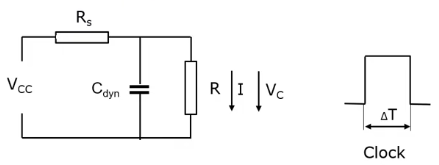
\includegraphics[width=0.8\textwidth]{dyndis}
    \centering
    \caption{Aktív tranzisztorok modellje}
    \label{fig:dyndis}
\end{figure}
Ebből a dinamikus disszipáció kiszámítása:
\begin{equation}
    D_d=2*C_dyn*V_cc^2*f_c
\end{equation}
Az órafrekvenciával lineáris, mivel a töltés-kisülések mennyisége függ tőle.

\section{TDP}
Thermal Design Power, azaz tervezési hőérték.
Egy számításigényes alkalmazás futtatása közbeni maximális disszipációt jelenti.
Fontos, hogy nem teljesen pontos érték.
Az OEM-ek ez alapján tervezik a hűtés rendszereket, aminek legalább ezt a TDP értéket el kell vezetnie úgy, hogy a tranzisztorok hőmérséklete nem megy kb. 80-90°C fölé.
A kategóriák jellemző TDP értékeit mutatja a \ref{fig:tdp}. ábra.
\begin{figure}[H]
    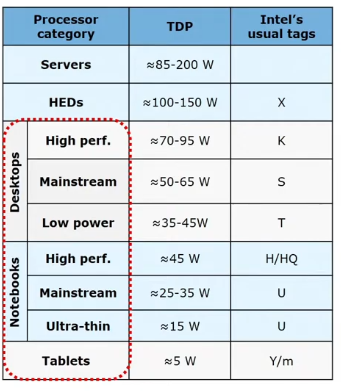
\includegraphics[width=0.6\textwidth]{tdp}
    \centering
    \caption{Processzor osztályok jellemző disszipációja}
    \label{fig:tdp}
\end{figure}
A TDP korlátozza az alapfrekvenciát.
A Turbo működéséhez jóval több watt szükséges.

\section{Intel processzorok disszipációja a fejlődés során}
A \ref{fig:evointel}. ábrán az Intel processzorok lapkamérethez viszonyított disszipációjának növekedése látható az órajel növekedésével.
\begin{figure}[H]
    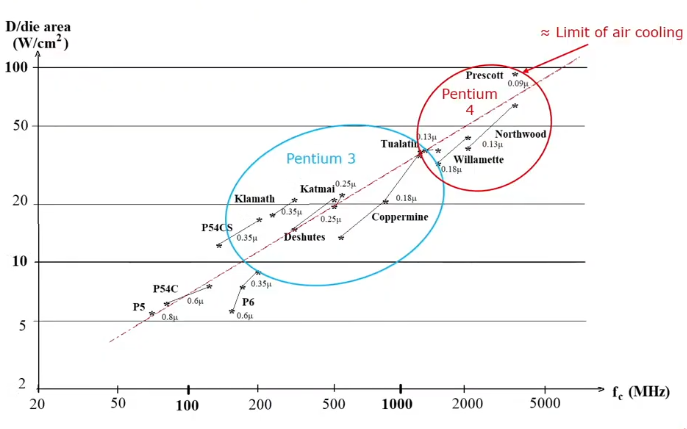
\includegraphics[width=0.8\textwidth]{evointel}
    \centering
    \caption{Disszipáció változása az órajel függvényében}
    \label{fig:evointel}
\end{figure}
Látható, hogy a Pentium 4 Prescott mag már közel 100 wattot adott le cm\textsuperscript{2}-enként, ami a léghűtés fizikai határa.
Az Intel 2000-ben azt várta a Pentium 4 családtól, hogy 10 évig gyártásban marad és 10 GHz órajelet fog elérni.
Ehelyett 2004-ben 4 GHz-nél megakadt a fejlesztés.
A Prescott család bizonyos tagjait kénytelenek voltak visszavonni túlmelegedési problémák miatt.

Ezzel az Intel 2003-tól a nyers teljesítményről áthelyezte a hangsúlyt a teljesítmény per watt, azaz a hatékonyság növelésére.
Összefoglalva a tervezési paradigmák változását mutatja a \ref{fig:paradigm}. ábra.
\begin{figure}[H]
    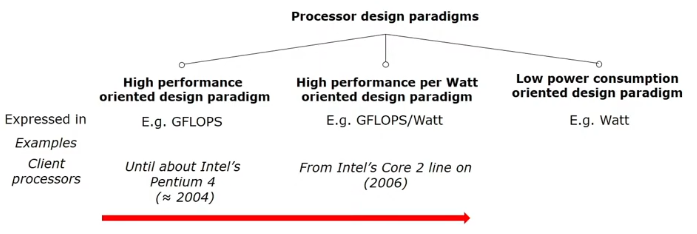
\includegraphics[width=0.8\textwidth]{paradigm}
    \centering
    \caption{Processzor tervezési paradigmák}
    \label{fig:paradigm}
\end{figure}

\section{Disszipációcsökkentő kezdeményezések}
A disszipáció kezelésére megszületett az Energy Star kezdeményezés, az AMD pedig célul tűzte ki, hogy 2014 és 2020 között 20x-osára emeli a hatékonyságot.

\subsection{Energy Star}
Az amerikai környezetvédelmi hatóság indította 1992-ben, az energiatudatosság elterjesztésére a processzoroknál.
Több verziója volt, a legfontosabb az 5., amit 2009-ben adtak ki, a Pentium 4 problémái után.
Lényege, hogy a processzorokra kiszámítják az éves inaktív állapotú energiafogyasztást, és ha egy modell a határérték alatt van, akkor használhatja az Energy Star jelölést.
A különböző inaktív állapotok súlyozása kategóriánként eltér.

\subsection{Az AMD hatékonysági kezdeményezése}
2014-ben jelentették be, hogy növelni szeretnék a teljesítmény per watt arányt.
2009-től 2014-ig 10x-es hatékonyság növekedést értek el, ehhez képest szerettek volna további 25x-ös javulást 2020-ra.
2020-ban bejelentették, hogy a Zen 2 alapú Ryzen processzoraikkal elérték a célt, 32x-es növekedéssel.

\subsection{Szerverek energiahatékonysága}
A szervereknél kiemelten fontos a hatékonyság, mivel egy adatközpont több MW áramot is fogyaszthat.
A szuperszámítógépeket hatékonyság szerint is rangsorolják, erre szolgál a Green500-as lista.

\section{ACPI}
Az inaktív állapot definiálása az Energy Star-hoz az ACPI (Advanced Configuration and Power Interface) szabvány segítségével lehetséges.
Ez egy nyílt szabvány, ami definiálja a számítógép állapotait.
Az állapotot globális (Gi), teljesítmény (Pi), inaktív (Ci) és alvó (G3) állapotok jellemzik (\ref{fig:acpi}. ábra).
\begin{figure}[H]
    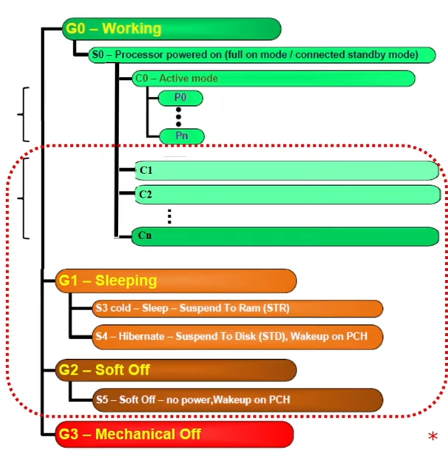
\includegraphics[width=0.5\textwidth]{acpi}
    \centering
    \caption{ACPI állapotok}
    \label{fig:acpi}
\end{figure}

Globális állapotok:
\begin{itemize}
    \item G1: OS által kezdeményezett leállás, kontextus mentéssel
    \item G2: OS által kezdeményezett leállás, kontextus mentés nélkül, tápellátás megmarad
    \item G3: mechanikai kikapcsolás
\end{itemize}

\section{A disszipációkezelés technikái}
A disszipáció kezelése sokféleképpen történhet, a tranzisztorok tervezésétől az áramkörökön és a processzoron át egészen a platform és operációs rendszer szintekig.

\subsection{Kezelés CPU szinten}
Kétféle kezelési lehetőség:
\begin{itemize}
    \item aktív magok kezelési technikái:
    \begin{itemize}
        \item energiafogyasztás csökkentése:
        \begin{itemize}
            \item DVFS - dinamikus feszültség és frekvencia kezelés
            \item CPPC
            \item AVFS - adaptív feszültség és frekvencia kezelése
        \end{itemize}
        \item Turbo Boost: a TDP hőtartalékát felhasználva megemeli a processzor az alap frekvenciáját ideiglenesen
    \end{itemize}
    \item inaktív magok kezelési technikái (ACPI alapú, C állapoton keresztül): a kihasználatlan magot egyre mélyebb alvó állapotba helyezi a rendszer.
\end{itemize}

\subsection{Kezelés áramköri szinten}
Két jelentős technológia:
\begin{itemize}
    \item óra kapuzás
    \item tápfeszültség kapuzás
\end{itemize}

\subsubsection{Óra kapuzás}
Az éppen inaktív áramkörök elé egy AND kapu kerül, ami inaktivitás esetén nem küld órajelet az áramkörre, így csökkentve a fogyasztást.
A statikus disszipáció viszont továbbra is fennmarad.
Implementációja történhet finom vagy durva szemcsézettséggel.
A finomnál kis áramköri egységeket külön-külön kapuznak, míg a durva szemcsézés több modult kapuz egyszerre.
Az óra kapuzást korán, már 1996-ban is alkalmazta a DEC cég az Alpha processzoraiban (lebegőpontos egységeket kapuzták).
Mivel a technológia jól bevált, hamar elterjedt, az Intel a Pentium 4-től használja, ma már teljesen általános.

\subsubsection{Tápellátás kapuzása}
Az óra kapuzás továbbfejlesztése, nagyobb áramköri egységekre használják mint pl. mag vagy memória kontroller.
Az egység inaktivitása esetén a komplett tápellátást lekapcsolja az egységről, így a dinamikus és a statikus disszipációt is megszüntetve.
A többmagos processzorokban a processzormagok külön-külön kapuzhatók.

A tápfeszültség kapuzás előfeltétele a Turbo Boost technológiának, mivel a Turbo órajel a processzor fogyasztása és a TDP közötti hőtartalékot felhasználva emeli meg az órajelet.
Ehhez elegendő hőtartalékot kell biztosítani, amit nagyban elősegít a kapuzás.

A tápellátás kapuzást az Intel vezette be a Nehalem processzorokkal 2008-ban.
Később az AMD és az IBM is átvette.

Implementáció szerint először (Nehalem) csak a magokat kapuzták, később több egységre is kiterjedt mint pl. L3 cache, GPU, memória kontroller.
Az Intel a Westmere, Sandy Bridge és Ivy Bridge folyamatosan terjesztette ki a kapuzást, az AMD a Bulldozer családdal gyakorlatilag minden alapegységet kapuzott.

A tápellátás megszüntetése történhet a pozitív pólus vagy a föld elvágásával is.

\subsubsection{Integrált tápegységek - Intel FIVR}
Az Intel a Haswell családdal továbbfejlesztette az energiaellátást, a tápegység (voltage regulator) bizonyos részeinek processzorlapkára helyezésével.
Ez a FIVR (Fully Integrated Voltage Regulator), ami eltérő feszültséggel tudja ellátni a processzor különböző részeit, így a kapuzás fölöslegessé vált.

Ezt a technológiát a Haswell és Broadwell processzorok után felfüggesztették, mivel az integrált tápegység a processzor disszipációjához adott hozzá, így csökkentve az elérhető órajelet.
A Skylake-el kezdődően tehát ideiglenesen visszatértek a teljesítmény kapuzásra.

\subsubsection{Feszültség lekapcsolás előkészítése}
Mielőtt egy magról lekapcsolnánk a tápot, a gyorsítótárat vissza kell írni a következő szintű gyorsítótárba, vagy ha az nem elérhető, memóriába.
A processzor végrehajtási állapotát (kontextus, azaz a regiszterek állapota) is el kell menteni egy következő szintű cache-be, vagy a memóriába, esetleg SRAM-ba.
A táp lekapcsolással együtt a magról lekapcsolják az órajelet és az órajel generátort is.

\subsubsection{A kontextus mentése}
A kontextus mentése történhet:
\begin{itemize}
    \item memóriába (AMD használta pl. Bulldozer, Piledriver, Excavator, Bobcat, Jaguar)
    \item következő szintű gyorsítótárba (AMD Jaguar, Puma)
    \item magonkénti SRAM-ba (Intel processzorok)
\end{itemize}

\subsection{Kezelés platform szinten}
Platform szinten bonyolult a disszipáció kezelés, mivel részt vesz benne a processzor, az IO eszközök, a BIOS és az OS is.
Az első ilyen megoldások az Inteltől származnak (SL), később a Microsofttal összefogva fejlesztettek (APM, nem terjedt el).
Később több gyártó is bekapcsolódott, így alakult ki a nyitott ACPI szabvány (1996-tól máig használják).

\subsubsection{Az ACPI fejlődése}
Az ACPI 1.0 verziót a Windows 95, 98, 2000 és NT 4.0 rendszerek támogatták.
Az XP és a Server 2003 rendszerek már az ACPI 2.0-t használták, amiben már jelen volt a DVFS (Dynamic Voltage and Frequency Scaling) és nagyban elősegítette a disszipáció kezelését.
A többmagos és többszálas rendszerek támogatása az ACPI 3.0-ban jelent meg, ezt a Vista, 7 és Server 2008 operációs rendszerek használták.
A 4.0 kevésbé jelentős, de az 5.0 egy új szemléletet vezetett be: Collaborative Processor Performance Control, aminek során az operációs rendszer csak átadja a processzornak, hogy a felhasználó a teljesítményt vagy az alacsony fogyasztást preferálja, majd ezután a többi döntést a processzor hozza meg hardveresen.
A fejlődés folytatódott, de a 6-os verziónak nem voltak jelentős újításai.